%!TEX root = ../swiatlow_thesis.tex
\label{chapter:lhc}

The Large Hadron Collider (LHC) is a 27 km long proton-proton ($pp$) synchotron built on the border of France and Switzerland, near the city of Geneva. The accelerator is nestled beneath mostly bucolic French farmland, as seen in Figure~\ref{fig:lhc:cern-lhc-aerial}.

%%%%%%%%%%%%%%%%

\begin{figure}
\centering
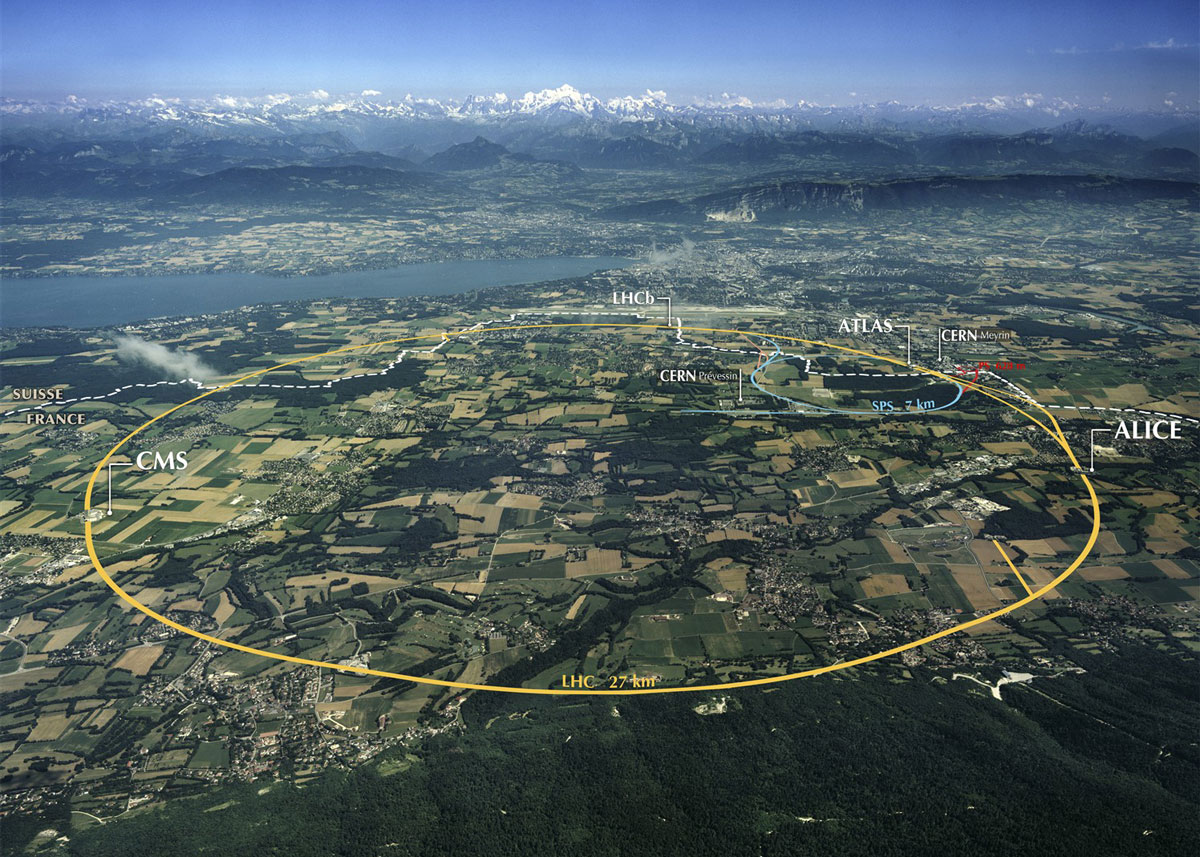
\includegraphics[width=0.8\textwidth]{cern-lhc-aerial.jpg}
\label{fig:lhc:cern-lhc-aerial}
\caption{An aerial view of Geneva, with the location of the LHC superimposed. The individual detectors (described in chapter~\ref{chapter:detector}, as well as the main CERN Meyrin site, are also highlighted. Image courtesy CERN.}
\end{figure}

%%%%%%%%%%%%%%%% 

The total costs of the accelerator and the detectors it serves are estimated at \$20 billion, making the LHC one of the largest scientific enterprises ever attempted. \editnote{cite this} The project is full of similar superlatives: the accelerator is the largest machine, the ATLAS detector is the largest detector, the CMS detector is the heaviest. 10,000 scientists from 113 countries work on some aspect of the project, making it one of the best examples of international cooperation that mankind has produced.



The machine was designed to deliver collisions at $\sqrt{s} = 14$~\TeV~energy at a rate of $10^{34}$~\lumirate, but as of 2012 collisions had only occured at 8 \TeV and a rate of $5\times10^{33}$~\lumirate. 

\editnote{Describe sectors, luminosity, energy, helium}



\section{History}
\label{lhc:history}

The LHC was first discussed publically at the ECFA-CERN Workshop held at Lausanne and Geneva in March of 1984~\cite{ECFA1984}\footnote{4 years and 1 month before the author was born!}. This was a very active time for proposing new collider experiments, as extensive work on the 40~\TeV $pp$ Superconducting Supercollider (to be built in Waxahachie, Texas) had recently displaced a proposal for a 4~\TeV~$p\bar{p}$ Dedicated Collider at Fermilab~\cite{ECFA1984,DC}, though construction continued on Fermilab's 2~\TeV~$p\bar{p}$ Tevatron collider. The Soviet Union was even planning a 6~\TeV~$p\bar{b}$ collider, the Accelerator and Storage Complex (UNK)~\cite{UNK}\editnote{This needs a better citation}. In this busy landscape, the proposal of another machine at CERN-- which was currently building the Large Electron Positron (LEP), the world's largest $e^+/e^-$ collider-- was very ambitious indeed.

Several characteristics made the proposed LHC unique and worth pursuing in such a competitive environment. First, with the construction of the LEP tunnel on track for completion in 1988, the civil-engineering component of the project was greatly reduced, especially compared to the enormous expense of constructing the SSC tunnel. Second, while the design goals of 20~\TeV~collisions were at a significantly lower energy than the SSC, the projected luminosity was eventually designed to be a factor of 10 higher (10$^{34}$~\lumirate, though the initial designs focused on 10$^{33}$~\lumirate) and so the LHC could potentially gain sensitivity by accumulating data more quickly. Finally, as figure \ref{fig:lhc:lep-lhc} shows, the initial designs for the LHC invisaged the LHC beamlines actually sitting on top of the existing LEP beamlines. The resulting hybrid collider would be able to run $pp$, $ep$, and $ee$ collisions. This would not only extend the reach of the physics program by allowing for the study of deep inelastic scattering at higher energies than the HERA collider at DESY \editnote{Cite this-- HERA and $e/p$ if possible.}, but would also allow for the study of $Z$ bosons from $ee$, which could potentially be used as a calibration source for detectors before $pp$ collisions~\cite{ECFA1984}.

%%%%%%%%%%%%%%%%

\begin{figure}
\centering
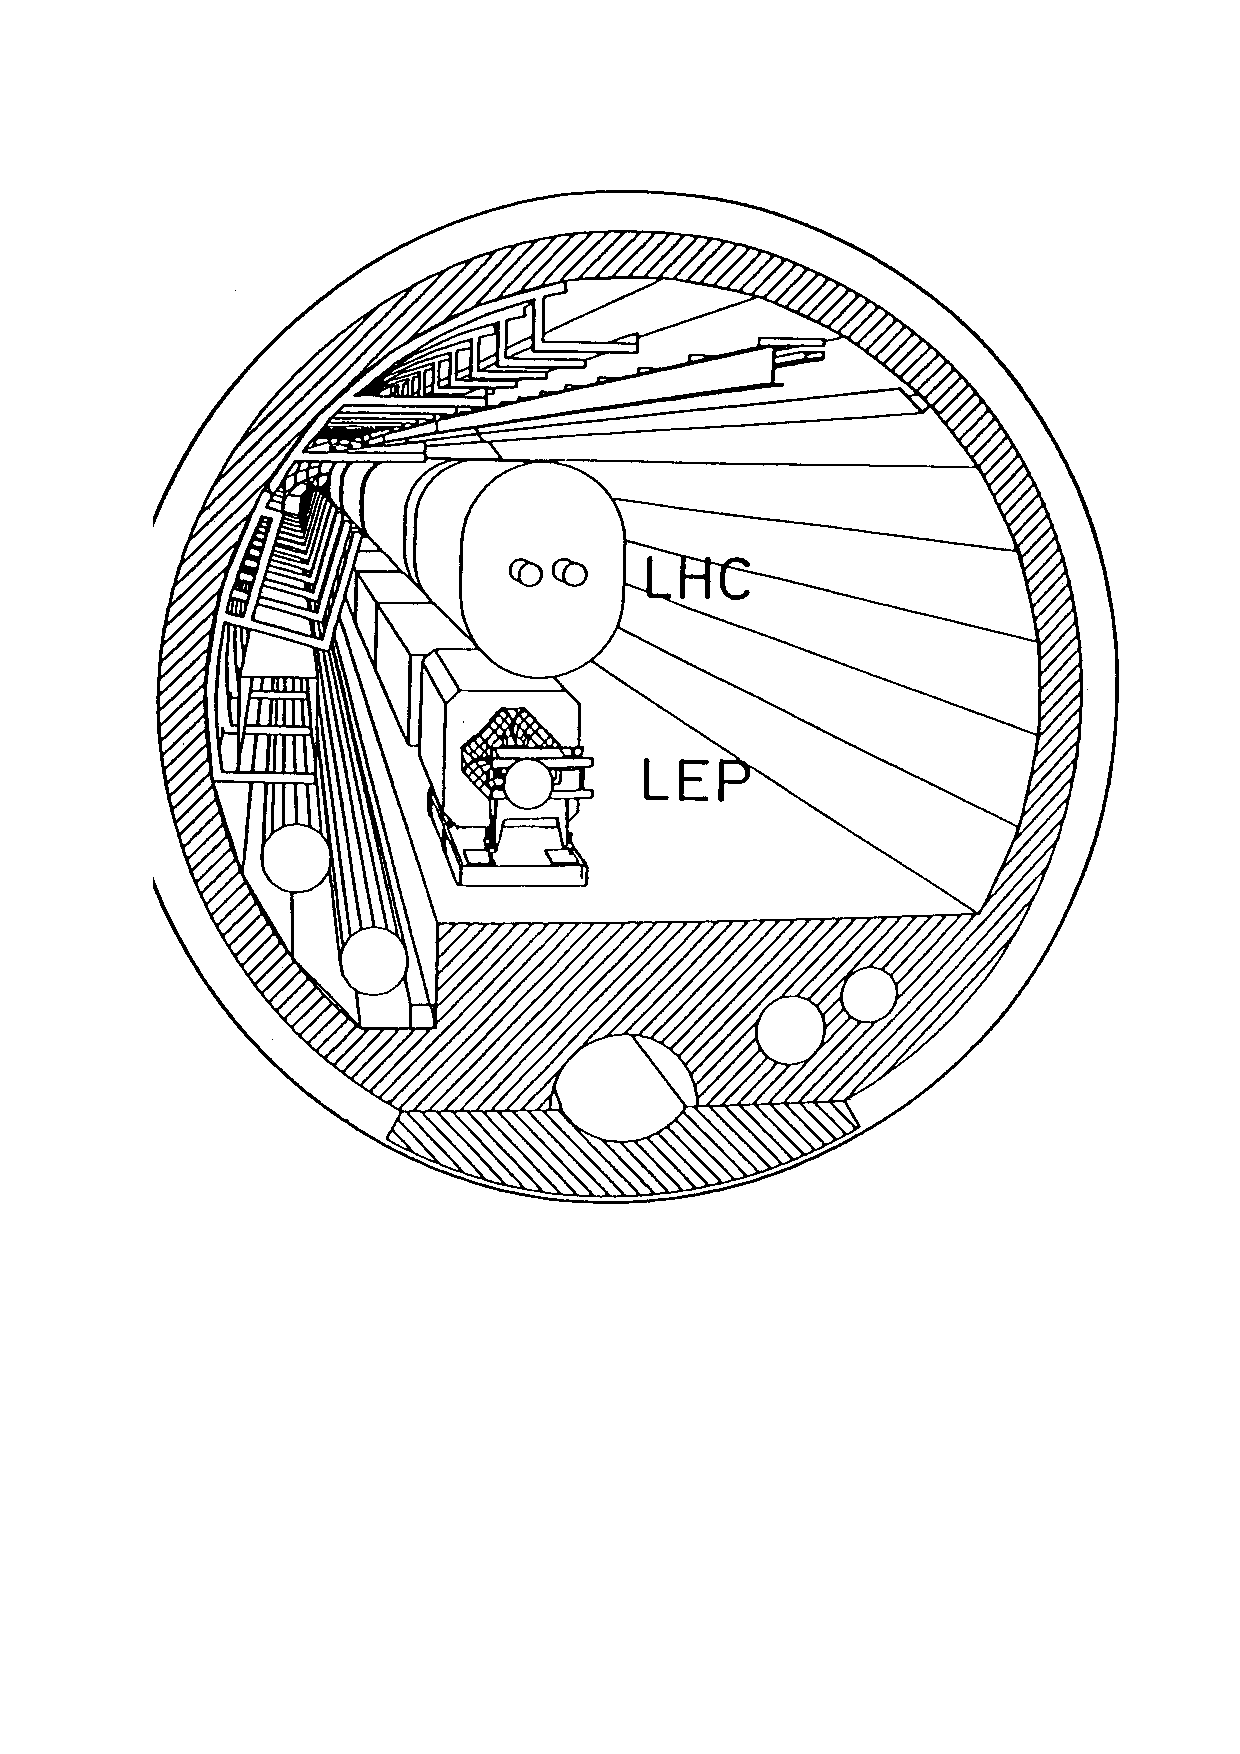
\includegraphics[width=0.8\textwidth]{lep-lhc.pdf}
\label{fig:lhc:lep-lhc}
\caption{A schematic drawing of the initial design of a shared LEP/LHC tunnel, with the LHC beamline positioned on top of the existing LEP beamline~\cite{ECFA1984}.}
\end{figure}

%%%%%%%%%%%%%%%% 

With the approval of the SSC in 1987 and the subsequent start of construction in 1991, CERN was mostly focused on the construction and operation of LEP but did not stop planning for the LHC. This proved remarkly prescient, as in the face of changing budget priorities and the end of the Cold War, the SSC ended up being cancelled in 1993. \editnote{This probably needs citations.} CERN, on the other hand, approved a staged construction plan for the LHC in 1994, targetting first 10~\TeV~collisions in 2004 and then 14~\TeV~in 2008. Japan and the US joined CERN as observer states in 1995 and 1997 respectively, each contributing signficantly to the construction of the LHC and joining the physics program of CERN.\editnote{Statement about internation collaboration, compared to SSC? Statement about the 10 TeV plan being dropped?}

The Conceptual Design Report~\cite{LHCCDR} published in 1995 reflected the changed landscape with the demise of the SSC and the results of more detailed cost estimates. The design energy was lowered to 14~\TeV-- higher energies would have required more costly magnets-- while the design luminosity was actually increased to 10$^{34}$~\lumirate. This increase in luminosity came at a cost: the number of interaction points was reduced to four instead of eight, and only two would receive collisions at a high rate. \editnote{Mention pileup here or no?} Critically, it was also decided to remove the LEP beamline and magnets, as it was deemed too costly to follow the existing LEP infrastructure. While this reduced the physics program of the LHC substantially, being the only high energy hadron collider was still a rather broad portfolio. For budgetary reasons, the initial proposal was for a two-stage design, with the first stage operating with only two-thirds the dipoles and therefore a lower energy.

Non-member states joined the proposal quickly: Japan contributed in 1995; India, Russia, and Canada joined in 1996; and the US became a partner in 1997. This financial outlook for the LHC was still not completely safe, as Germany (and later the UK) unilaterally reduced their contribution to CERN between 8-9$\%$. This issue was resolved by allowing CERN to take on debt to finance the entire project in one construction phase-- a decision which raised the total cost of the LHC by $20\%$.


With the shutdown of LEP in 2001\footnote{Not without controversy, as there was perhaps a tantalizing sign of an excess in Higgs-boson like events during the final runs of LEP.\editnote{cite me}}, the construction of the LHC began in earnest. It would take till 2007 to install the last magnet in the LHC, and the detectors finalized their own installations only in 2008. Figure~\ref{fig:lhc:lhc-tunnel} shows the final state of the LHC tunnel (without the originally planned LEP beamline). The first low-energy collisions occured on September 10, 2008, putting the LHC almost on track of its initial goal of 14~\TeV collisions in 2008. \editnote{Probably want to add a bit more on construction.}

%%%%%%%%%%%%%%%%

\begin{figure}
\centering
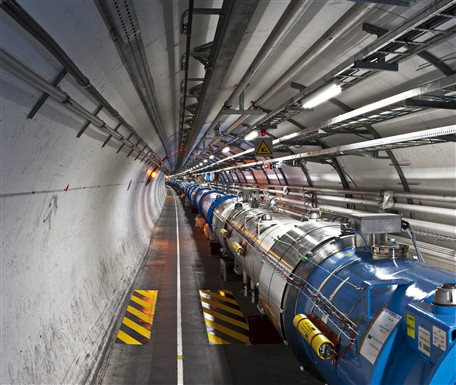
\includegraphics[width=0.8\textwidth]{lhc-tunnel.jpg}
\label{fig:lhc:lhc-tunnel}
\caption{A photo of the final LHC tunnel, no LEP beamline, in contrast to the first plans shown in Figure~\ref{fig:lhc:lep-lhc}. Photo courtesy of USLHC.}
\end{figure}

%%%%%%%%%%%%%%%% 

However, an ``incident'' on September 19 ended up delaying the full startup for a year~\cite{Incident}. On that day, the operators were testing the last sector of the LHC at current levels appropriate fo 5.5~\TeV beams. A resistive zone developed in the electrical bus connection between a dipole and quadrupole magnet. While the power supply detected this and shut down within 0.39 seconds and the quench protection circuitry began to engage at 0.89 seconds, it was already too late: an electrical arc had sparked and punctured the liquid helium enclosure and the insulation vacuum along the cryostat. This, along with the electrical noise induced by the power supply shutdown and the heat dissipation caused by the quench protection circuitry, triggered a chain reaction in which several other magnets also began to quench and other vacuum systems were degraded. As the helium began to escape the cryostat, pressure relief valves correctly opened and vented the helium to atmosphere. However, an additional complication proved to be a problem: neighboring subsectors had their vacuum systems separated by vacuum barriers, meant to isolate the vacuum systems of neighboring areas. The vacuum barriers could only sustain a rather low pressure difference, and the extreme pressures generated by the evacuating helium overwhelmed these connections. The attendant large pressure forces ended up displacing dipoles from their support structures, and knocked the cryostats from their support jacks-- in some cases even ripping the anchors from the concrete floor. A total of six tons of helium, five quadrupoles, and twenty-four dipoles were lost in the incident. 

The damage to the accelerator was repaired in 2009, and on November 20, 2009, 450 GeV protons from the Super Proton Synchotron were injected into the LHC for the first time since the incident. November 23rd saw the first $pp$ collisions in all four LHC detectors, albeit at only $\sqrt{s} = 900$~\GeV. Several very short runs at this energy and $\sqrt{s} = 2.36$~\TeV followed, before the first $\sqrt{s} = 7$~\TeV collisions occured on March 30, 2010. It was decided to operate the LHC for several years at this lower energy, as more accelerator upgrades and consolidation would be required to safely operate at $\sqrt{s} = 14$~\TeV. 2010 saw a peak luminosity of only $2\times10^{32}$~\lumirate as the accelerator only very gradually increased the collision rate. 2011 saw delivery at a peak of $4 \times 10^{33}$~\lumirate-- only three times lower than the design luminosity.

After two years of successful and safe operations at the reduced energy, 2012 saw a large increase in luminosity-- to a peak of $8\times10^{33}$~\lumirate-- and an increase of the collision energy to 8~\TeV. The LHC then proceeded to shut down in 2013 until mid-2015 for a further round of repairs and consolidations of electrical connections to guarantee the safety of operations at near the design energy. As the restart of the LHC approaches in the coming months, we are anticipating collisions at 13~\TeV with luminosity likewise reaching near design levels. The LHC will have broken energy records twice in the span of five years, making this an incredibly exciting time to be working in particle physics.


\section{Machine Design}

The LHC is the last of a long chain of accelerators used to accelerate ordinary protons obtained from hydrogen gas\cite{cern-accelerators}. The entire accelerator complex is shown in Figure~\ref{fig:lhc:cern-accelerators}. Protons from a simple bottle of hydrogen gas are stripped of their electrons in an electric field and are injected into the chain at the Linac2, which accelerates the particles to 50 MeV. The Proton Synchotron Booster (PSB) then accelerates the particles to 1.4 GeV, and sends them off to the Proton Synchotron (PS) to be accelerated to 25 GeV. The Super Proton Synchotron (SPS) then accepts the protons and accelerates them to 450 GeV, which is the energy of injection at the LHC. The injection process per beam takes 260 seconds, and then another 20 minutes is required to raise the energy to collision levels.

%%%%%%%%%%%%%%%%

\begin{figure}
\centering
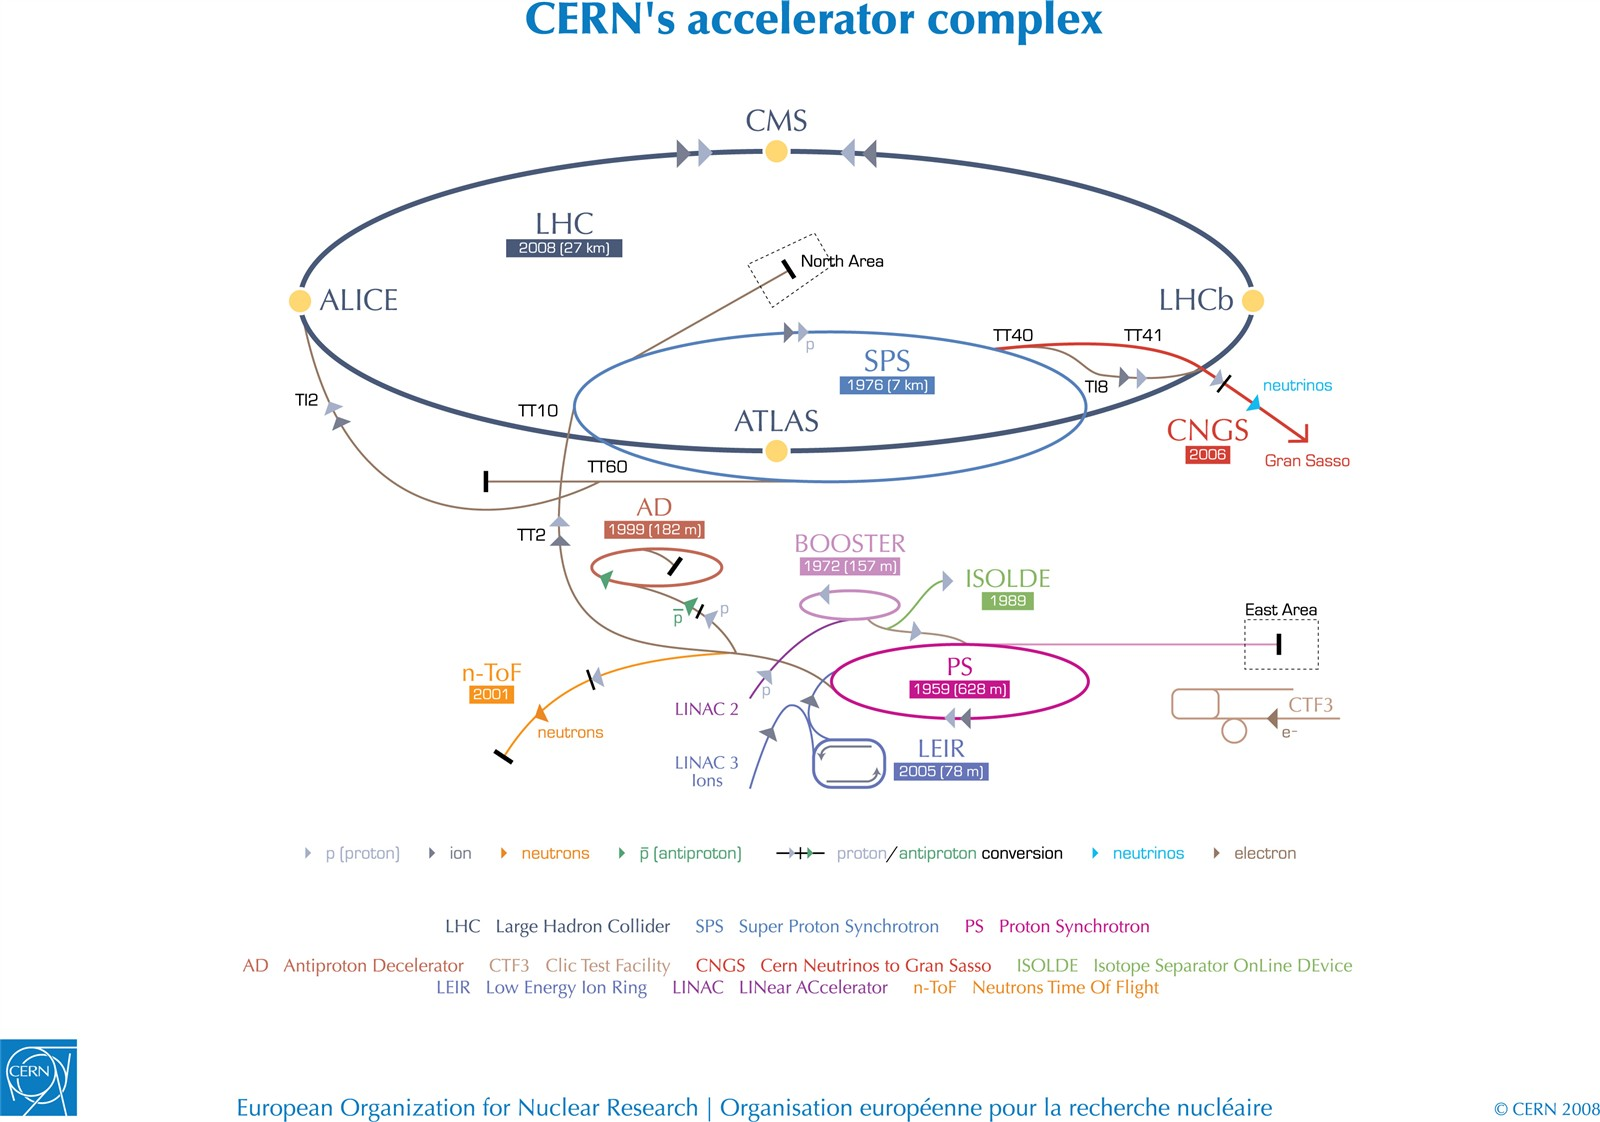
\includegraphics[width=0.8\textwidth]{cernaccelerators.jpg}
\label{fig:lhc:cern-accelerators}
\caption{A diagram of the CERN accelerator chain, with each accelerator listing both its year of completion and length. Copyright CERN.}
\end{figure}

%%%%%%%%%%%%%%%% 

Each stage of the chain accelerates particles by a factor of between 10-20 times their energy. This is a consequence of the fixed bending radius in an accelerator, $\rho$, which is~\cite{accelerator-book}:
%
\begin{equation}
\frac{1}{\rho} (\mathrm{m}^{-1}) = 0.2998 \frac{|B (\mathrm{T})|}{\beta E (\GeV)}.
\end{equation}
%
As the bending radius is fixed, this means that as the energy of the beam goes up, the magnetic field must go up linearly to keep the particles inside the ring. This also means that as particles are injected from one accelerator to another (and the radius therefore increases), the magnetic field must be the same factor smaller. The lower range of practical bending magnet strength is set by stray magnetic fields in the earth; the upper range is set by the material of the magnet and energy consumption. These restrictions (how weak the magnets can be during injection, and how strong after acceleration) limit each stage of the accelerator chain to increasing the energy by a factor of $\approx$200. In practice, the accelerating factor is lower (10-20), because it is much easier to not use the full range of the magnet strength (particularly at the low end), and the size of each accelerator is not designed optimally but instead historically, as each accelerator was previously used for collisions at a lower energy. For example, the SPS could have been ejected particles at a much lower energy and the LHC accepted them by using a lower initial field strength, but as the SPS was already built, the operation of the LHC is simplified by using a higher initial field. \editnote{This might need revision}



The machine is composed of eight essentially identical sectors, 

\section{Luminosity, and Pileup}
\label{lhc:luminosity-and-pileup}

\section{Operations in 2010-2012}